\documentclass{article}

\usepackage[portuguese]{babel}

\usepackage[letterpaper,top=2cm,bottom=2cm,left=3cm,right=3cm,marginparwidth=1.75cm]{geometry}

% Useful packages
\usepackage{amsmath}
\usepackage{graphicx}
\usepackage[colorlinks=true, allcolors=blue]{hyperref}

\title{Modelos de aprendizado de máquina aplicados à detecção de fraudes bancárias}
\author{Cristiano Mendieta, Gabrielly Halas, Kléber Benatti, Mateus Fernandes}

\begin{document}
\maketitle

%----------------------------------------------------------------------------------------------------------
\begin{abstract}
[inserir]
\end{abstract}


%----------------------------------------------------------------------------------------------------------
\section{Introdução}

[inserir]
Principais desafios:

\begin{enumerate}
    \item Muitos padrões de fraude;
    \item Mudança de tendência nas fraudes;
    \item Automação em \textit{real time};
    \item Classes desbalanceadas (poucas fraudes para muitas transações fidedignas);
    \item Órgãos reguladores exigem interpretabilidade em alguns cenários.
\end{enumerate}

Serão abordados problemas (1), (4) e (5) no projeto, a partir do estudo de:

\begin{itemize}
    \item Modelos interpretáveis: Árvores de Decisão e Regressão Logística.
\end{itemize}


%----------------------------------------------------------------------------------------------------------
\section{Análise exploratória dos dados e dataprep}

A base de dados utilizada na implementação dos modelos foi extraída do \textit{Kaggle}, plataforma que armazena e disponibiliza diversos \textit{datasets} e permite hospedar competições de \textit{Data Science}, tanto patrocinadas quanto focadas no aprendizado.

Foi escolhido o \textit{dataset} \textit{Credit Card Transactions Fraud Detection Dataset}, que contém dados simulados de transações de cartão de crédito geradas usando \textit{Sparkov}, disponível por meio do link  \href{https://www.kaggle.com/kartik2112/fraud-detection?select=fraudTrain.csv}{https://www.kaggle.com/kartik2112/fraud-detection?select=fraudTrain.csv}. Ela é composta por dois arquivos no formato \textit{comma-separated values} (.csv): fraudTest.csv e fraudTrain.csv. Para melhor compreensão dessa base foi realizada uma análise exploratória.  

A base é formada 1296675 observações distribuídas em 23 variáveis, sendo 11 numéricas e 12 fatores, organizadas conforme segue:

\begin{itemize}
    \item index [numérica] - identificador único de cada linha;
    \item transdatetrans\_time [fator] - data e horário da transação;
    \item cc\_num [numérica] - número de cartão de crédito do consumidor, contando com 983 números únicos;
    \item merchant [fator] - nome do comerciante, contando com 693 nomes únicos;
    \item category [fator] - categoria do comerciante, contando com 14 diferentes categorias;
    \item amt [numérica] - valor da transação, sendo o mínimo de 1 e máximo de 28948,90, com média de 70,35;
    \item first [fator] - primeiro nome do titular do cartão de crédito;
    \item last [fator] - sobrenome do titular do cartão de crédito;
    \item gender [fator] - sexo do titular do cartão de crédito;
    \item street [fator] - endereço do titular do cartão de crédito;
    \item city [fator] - cidade do titular do cartão de crédito, conta 894 diferentes cidades;
    \item state [fator] - estado do titular do cartão de crédito, conta com 51 diferentes estados;
    \item zip [numérica] - zip do titular do cartão de crédito;
    \item lat [numérica] - latitude da localização do titular do cartão de crédito;
    \item long [numérica] - longitude da localização do titular do cartão de crédito;
    \item city\_pop [numérica] - população de titulares de cartão de crédito na cidade;
    \item job [factor] - profissão do titular do cartão de crédito, sendo 494 diferentes profissões;
    \item dob [factor] - data de nascimento do titular do cartão de crédito;
    \item trans\_num [factor] - número da transação;
    \item unix\_time [numérica] - UNIX time (representação da data da transação em segundos);
    \item merch\_lat [numérica] - latitude da localização do comerciante;
    \item merch\_long [numérica] - longitude da localização do comerciante;
    \item is\_fraud [numérica] - \textit{flag} que determina se a transação é (1) ou não (0) fraude. 
\end{itemize}

Não foram identificados dados duplicados, nem valores faltantes. Para facilitar a utilização dos dados, a coluna \textit{transdatetrans\_time} foi separada em duas: uma de data \textit{(date)} e uma de hora \textit{(time)}. Ademais, seguem observações obtidas a partir da exploração das variáveis \textit{category, amt, gender, city, job, lat, long, merch\_lat, merch\_long, is\_fraud}.


%----------------------------------------------------------------------------------------------------------
\subsection{Variáveis \textit{is\_fraud} e \textit{gender}}

Em relação ao total de 1296675 observações tem-se que 7506 delas foram classificadas como fraudes, ou seja, 0.5789\% do total de dados.

Do total de 1296675 transações tem-se que 45.255\% foram realizadas por pessoas do sexo masculino e 54.745\% por pessoas do sexo feminino, sendo que a taxa de fraudes se apresenta superior para as pessoas de sexo masculino, conforme é possível observar na tabela \ref{tab-gender}. 

\begin{table}[!ht]
\centering
\begin{tabular}{cccc}
Sexo      & Total Fraudes & Total de Observações & Taxa de fraudes \\ \hline
Masculino & 3771          & 586812               & 0.00643         \\
Feminino  & 3735          & 709863               & 0.00526        
\end{tabular}
\caption{Taxa de fraudes por sexo (FONTE: Autores(2022))}
\label{tab-gender}
\end{table}

%----------------------------------------------------------------------------------------------------------
\subsection{Variável \textit{category}}

Em relação a variável \textit{category}, que diz respeito as 14 categorias do comerciante que constam no conjunto de dados, tem-se que o gráfico \ref{graf-category} aponta que a maior taxa de de fraudes ocorreu em comércios categorizados em \textit{shopping\_net} (0.0176), \textit{misc\_net} (0.0145) e \textit{grocery\_pos} (0.0141).

\begin{figure}[!ht]
    \centering
    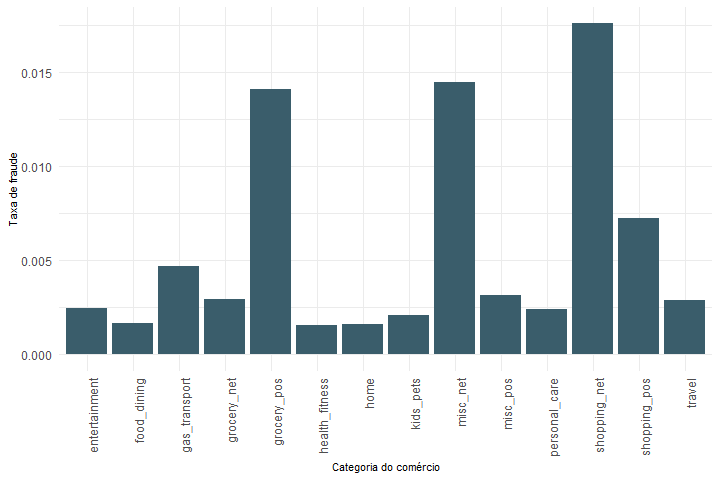
\includegraphics[scale = 0.5]{graf-category.png}
    \caption{Taxa de fraudes por categoria de comércio (FONTE: Autores (2022))}
    \label{graf-category}
\end{figure}

\newpage
Para auxiliar a utilização dessa variável nos modelos, as taxas de fraude relacionadas a ela cuja amplitude foi de 0.01607 foram distribuídas em 10 intervalos de amplitude 0.001607. A maior parte das taxas concentrou-se no intervalo ${[}0.00153,0.00315{]}$ (faixa 1), conforme observa-se na tabela \ref{tab-category}. A base foi acrescida de uma coluna \textit{faixascategory}, a fim de classificar os dados da coluna \textit{category} em suas respectivas faixas, de acordo com as taxas de fraude.

\begin{table}[!ht]
\centering
\begin{tabular}{ccc}
Faixa & Intervalo             & Quantidade de taxas \\ \hline
1     & {[}0.00153,0.00315{]} & 9                   \\
2     & (0.00315,0.00475{]}   & 1                   \\
3     & (0.00475,0.00635{]}   & 0                   \\
4     & (0.00635,0.00795{]}   & 1                   \\
5     & (0.00795,0.00956{]}   & 0                   \\
6     & (0.00956,0.0112{]}    & 0                   \\
7     & (0.0112,0.0128{]}     & 0                   \\
8     & (0.0128,0.0144{]}     & 1                   \\
9     & (0.0144,0.016{]}      & 1                   \\
10    & (0.016,0.0176{]}      & 1                  
\end{tabular}
\caption{Faixas de taxas de fraude por categorias de comércio (FONTE: Autores (2022)).}
\label{tab-category}
\end{table}


%----------------------------------------------------------------------------------------------------------
\subsection{Variável \textit{job}}

A variável \textit{job} que traz a profissão dos titulares do cartão de crédito, aponta que das 494 diferentes profissões, as 10 com maior taxa de fraude foram \textit{Accountant, chartered; Air traffic controller; Armed forces technical officer; Broadcast journalist; Careers adviser; Contracting civil engineer; Dancer; Engineer, site; Forest/woodland manager; Homeopath.}

Assim como a variável \textit{category}, a variável \textit{job} também teve suas taxas de fraude organizadas em 10 intervalos. Ao distribuir a amplitude do conjunto em 10 intervalos de mesmo tamanho, percebeu-se uma grande concentração dos dados nos intervalos [0,0.1] e (0.9,1]. Dessa forma, os intervalos foram organizados em 0 a 0.000483, 8 faixas de igual amplitude entre 0.000483 e 0.0519, e um intervalo de 0.0519 a 1, obtendo-se as faixas conforme tabela \ref{tab-job}. A base foi acrescida de uma coluna \textit{faixasjob}, a fim de classificar os dados da coluna \textit{job} em suas respectivas faixas, de acordo com as taxas de fraude.

\begin{table}[!ht]
\centering
\begin{tabular}{ccc}
Faixa & Intervalo            & Quantidade de taxas \\ \hline
1     & {[}0,0.000483{]}     & 51              \\
2     & ({0.000483,0.0069]}  & 214             \\
3     & ({0.0069,0.0133]}    & 155             \\
4     & ({0.0133,0.0197]}    & 35              \\
5     & ({0.0197,0.0262]}    & 12              \\
6     & ({0.0262,0.0326]}    & 4               \\
7     & ({0.0326,0.039]}     & 1               \\
8     & ({0.039,0.0454]}     & 2               \\
9     & ({0.0454,0.0519]}    & 0               \\
10    & ({0.0519,1]}         & 20                
\end{tabular}
\caption{Faixas de taxas de fraude por profissão (FONTE: Autores (2022)).}
\label{tab-job}
\end{table}


%----------------------------------------------------------------------------------------------------------
\subsection{Variável \textit{city}}

A variável \textit{city} que contempla 894 diferentes cidades aponta que as 10 cidades com maior taxa de fraude foram Angwin, Ashland, Beacon, Brookfield, Bruce, Buellton, Byesville, Chattanooga, Clarion e Claypool. 

Da mesma forma como a variável \textit{job}, a variável \textit{city} também teve suas taxas de fraude organizadas em 10 intervalos. Ao distribuir a amplitude do conjunto em 10 intervalos de mesmo tamanho, também percebeu-se uma grande concentração dos dados nos intervalos [0,0.1] e (0.9,1]. Dessa forma, os intervalos foram organizados em 0 a 0.000394, 8 faixas de igual amplitude entre 0.000394 e 0.0449, e um intervalo de 0.0449 a 1, obtendo-se as faixas conforme tabela \ref{tab-city}. A base foi acrescida de uma coluna \textit{faixascity}, a fim de classificar os dados da coluna \textit{city} em suas respectivas faixas, de acordo com as taxas de fraude.

\begin{table}[!ht]
\centering
\begin{tabular}{ccc}
Faixa & Intervalo             & Quantidade de taxas \\ \hline
1     & {[}0,0.000394{]}      & 193                  \\
2     & ({0.000394,0.00596]}  & 248                 \\
3     & ({0.00596,0.0115]}    & 230                  \\
4     & ({0.0115,0.0171]}     & 69                 \\
5     & ({0.0171,0.0227]}     & 55                 \\
6     & ({0.0227,0.0282]}     & 31                 \\
7     & ({0.0282,0.0338]}     & 8                \\
8     & ({0.0338,0.0394]}     & 0               \\
9     & ({0.0394,0.0449]}     & 2                \\
10    & ({0.0449,1]}          & 58                
\end{tabular}
\caption{Faixas de taxas de fraude por cidade (FONTE: Autores (2022)).}
\label{tab-city}
\end{table}


%----------------------------------------------------------------------------------------------------------
\subsection{Variáveis \textit{lat, long, merch\_lat, merch\_long}}

Com o objetivo de calcular a distância geodésica entre o local de moradia do titular do cartão de crédito e o local no qual foi efetuada a transação, foram utilizadas as variáveis \textit{lat, long} referente a primeira localização citada e \textit{merch\_lat, merch\_long}, referente a segunda. Dessa forma, a base recebeu uma coluna \textit{distGeo} que conta com essas distâncias em metros.

%----------------------------------------------------------------------------------------------------------

\end{document}